\section{Exponentialfunktionen und Logarithmen}

Wir wollen uns nun mit Funktionen beschäftigen, die exponentielles Wachstum beschreiben. \emph{Exponentialfunktionen} sind Funktionen, deren Variable im Exponenten steht $f(x) = a^x$. Hierbei muss die Basis $a > 0$ sein. Unabhängig von $a$ gilt dann $a^0 = 1$, d.\,h. alle Exponentialfunktionen schneiden die $y$-Achse im Punkt $(0,1)$. 

Wir können, abhängig von $a$, drei Fälle unterscheiden 
\begin{itemize}
    \item $a > 1: \quad \lim_{x\to -\infty} a^x = 0$, asymptotische Annäherung an $x$-Achse von rechts
    \item $a < 1: \quad \lim_{x\to \infty} a^x = 0$, asymptotische Annäherung an $x$-Achse von links 
    \item $a = 1: \quad y=1$ für alle $x$
\end{itemize}

\begin{figure}[htp]
    \centering
    \begin{tikzpicture}
        \begin{axis}[disabledatascaling, axis lines=middle, xlabel={$x$}, ylabel={$y$}, height=7cm, width=0.9\textwidth, ymax=2.99, legend pos = outer north east, xmin=-1.1, xmax=1.1, ytick={2}]
            \addplot[no marks, FSUblau, thick, domain=-1:1]{2^x};
            \addplot[no marks, FSUblau, thick, dashed, domain=-1:1]{5^x};
            \addplot[no marks, PAForange, thick, domain=-1:1]{(1/2)^x};
            \addplot[no marks, PAForange, thick, dashed, domain=-1:1]{(1/5)^x};
            \addplot[no marks, Gruen, thick, domain=-1:1]{1};
            \node (A) at (-0.04,0.8){1};
            \legend{$a = 2 >1$, $a = 5 > 1$,$a = 1/2 <1$, $a=1/5 < 1$, $a=1$};
        \end{axis}
    \end{tikzpicture}
    \caption{Darstellung von Exponentialfunktionen für verschiedene Werte von $a$.}
\end{figure} 
Die Funktionen sind spiegelbildlich zur $x$-Achse, denn 
\begin{align}
    \begin{rcases}
        f_1(x) = a^x \\
        f_2(x) = \qty(\frac{1}{a})^x = a^{-x} = f_1(-x) 
    \end{rcases} \qq{wenn} a >1, \qq{dann} \frac{1}{a} < 1.
\end{align}
Das heißt, zu jeder \textcolor{FSUblau}{blauen} Funktion mit Basis $a$, findet man eine spiegelsymmetrische \textcolor{PAForange}{orangene} Funktion mit Basis $\frac{1}{a}$.

\subsection{Logarithmen}

Wir wollen uns nun die Frage stellen, welchen Wert $n$ ein Exponent zu einer gegebenen Basis $b$ haben muss, damit der Potenzwert $a$ herauskommt. Also es gelte $a = b^n$ für ein bekanntes $a$ und $b$, was ist dann $n$?

Die Antwort auf diese Frage liefert die Logarithmusfunktion: $(a,b > 0; b \neq 1)$
\begin{align}
    \tikzmarknode{eq1}{}n = \log_b\tikzmarknode{eq2}{}(\tikzmarknode{eq3}{}a).
\end{align}
\tikz[overlay,remember picture]{
\draw[shorten >=2pt,shorten <=2pt, thick, -{latex}] ($(eq2)+(0.8,-0.7)$)node[right]{Radikand} -- ($(eq2)+(-0.2,-0.1)$);
\draw[shorten >=2pt,shorten <=2pt, thick, -{latex}] ($(eq1)+(-0.7,0.1)$)node[left]{Exponent} -- ($(eq1)+(0,0.1)$);
\draw[shorten >=2pt,shorten <=2pt, thick, -{latex}] ($(eq3)+(1.3,0.15)$)node[right]{Numerus (Potenzwert)} -- ($(eq3)+(0.5,0.15)$);
}

Beispielsweise $n = \log_5(625)$ heißt, dass gilt: $5^n = 625$. Wir finden damit als Ergebnis $n=4$. Spezielle Werte des Logarithmus sind 
\begin{align}
    \begin{split}
        \log_b (1) &= 0 \qq{da} b^n = 1 \quad \Rightarrow \quad n=0\\
        \log_b (b) &= 1 \qq{da} b^n = b \quad \Rightarrow \quad n=1.
    \end{split}
\end{align}
Der Logarithmus ist die Umkehrfunktion der Exponentialfunktion. Es gilt demzufolge 
\begin{align}
    b^{\log_b(a)} = b^n = a \qq{und} \log_b(b^n) = \log_b(a) = n.
\end{align}
Beachte: Der Logarithmus von Null ist nicht definiert, da $10^b = 0$ keine reelle Lösung für $b$ hat. Ebenso ist der Logarithmus negativer Zahlen (hier) nicht definiert, da $10^b = x$ für $x <0$ keine reelle Lösung für $b$ hat.

\paragraph{Logarithmengesetze}$~$

Wir wollen im Folgenden die Logarithmengesetze aus den Potenzgesetzen herleiten: 

\begin{minipage}{0.5\textwidth}
    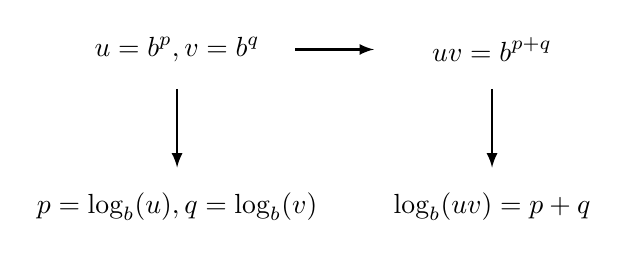
\begin{tikzpicture}
        \node (A) at (-2,1){$\displaystyle u = b^p, v = b^q$};
        \node (A) at (2,1){$\displaystyle  uv = b^{p+q}$};
        \node (A) at (-2,-1){$\displaystyle p = \log_b(u), q=\log_b(v)$};
        \node (A) at (2,-1){$\displaystyle \log_b(uv) = p+q$};
        \draw[thick, -{latex}] (-.5,1) -- (.5,1);
        \draw[thick, -{latex}] (-2,0.5) -- +(0,-1);
        \draw[thick, -{latex}] (2,0.5) -- +(0,-1);
    \end{tikzpicture}
\end{minipage}
\begin{minipage}{0.49\textwidth}
    \vspace{1.3cm}
    \begin{align}
        \Rightarrow \quad \log_b(uv) = \log_b(u) + \log_b(v).
    \end{align}
\end{minipage}

\begin{minipage}{0.5\textwidth}
    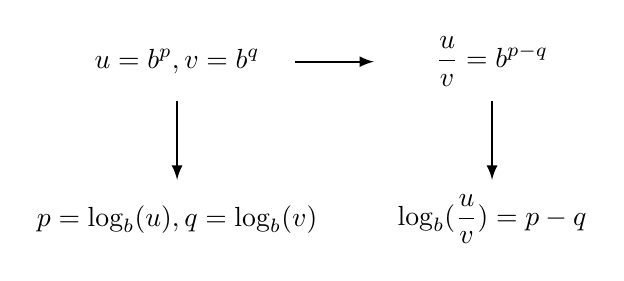
\begin{tikzpicture}
        \node (A) at (-2,1){$\displaystyle u = b^p, v = b^q$};
        \node (A) at (2,1){$\displaystyle  \frac{u}{v} = b^{p-q}$};
        \node (A) at (-2,-1){$\displaystyle p = \log_b(u), q=\log_b(v)$};
        \node (A) at (2,-1){$\displaystyle \log_b\qty(\frac{u}{v}) = p-q$};
        \draw[thick, -{latex}] (-.5,1) -- (.5,1);
        \draw[thick, -{latex}] (-2,0.5) -- +(0,-1);
        \draw[thick, -{latex}] (2,0.5) -- +(0,-1);
    \end{tikzpicture}
\end{minipage}
\begin{minipage}{0.49\textwidth}
    \vspace{1.4cm}
    \begin{align}
        \Rightarrow \quad \log_b\qty(\frac{u}{v}) = \log_b(u) - \log_b(v).
    \end{align}
\end{minipage}

\begin{minipage}{0.5\textwidth}
    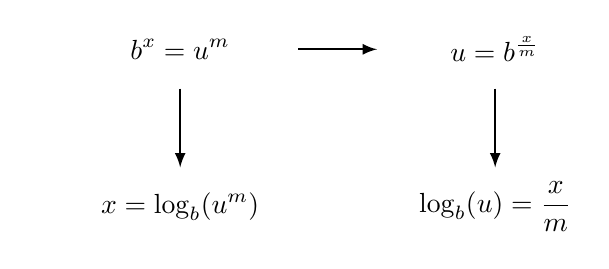
\begin{tikzpicture}
        \node (A) at (-3.82,1){};
        \node (A) at (-2,1){$\displaystyle b^x = u^m$};
        \node (A) at (2,1){$\displaystyle  u = b^{\frac{x}{m}}$};
        \node (A) at (-2,-1){$\displaystyle x = \log_b(u^m)$};
        \node (A) at (2,-1){$\displaystyle\log_b(u) = \frac{x}{m}$};
        \draw[thick, -{latex}] (-.5,1) -- (.5,1);
        \draw[thick, -{latex}] (-2,0.5) -- +(0,-1);
        \draw[thick, -{latex}] (2,0.5) -- +(0,-1);
    \end{tikzpicture}
\end{minipage}
\begin{minipage}{0.49\textwidth}
    \vspace{1.3cm}
    \begin{align}
        \Rightarrow \quad \log_b(u^m) = m \log_b(u).
    \end{align}
\end{minipage}

Die Logarithmus-Funktion wandelt Potenzen und Wurzeln in Produkte und Brüche und diese wiederum in Summen und Differenzen um.

\paragraph{Wechsel der Basis}$~$

Alle Logarithmen können bezüglich der gleichen Basis ausgedrückt werden. 

\begin{minipage}{0.5\textwidth}
    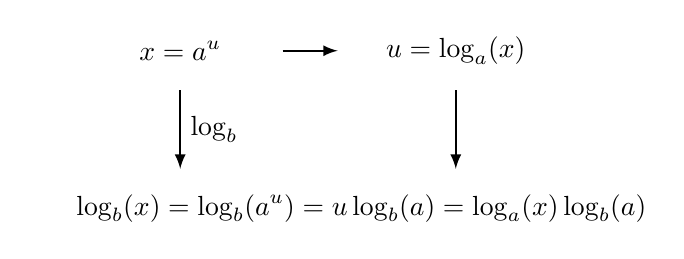
\begin{tikzpicture}
        \node (A) at (-3.82,1){};
        \node (A) at (-2,1){$\displaystyle x = a^u$};
        \node (A) at (1.5,1){$\displaystyle  u = \log_a(x)$};
        \node (A) at (0.3,-1){$\displaystyle \log_b(x) = \log_b(a^u) = u \log_b(a) = \log_a(x) \log_b(a)$};
        % \node (A) at (2,-1){$\displaystyle\log_b(u) = \frac{x}{m}$};
        \draw[thick, -{latex}] (-.7,1) --(0,1);
        \draw[thick, -{latex}] (-2,0.5) --node[right]{$\log_b$}  +(0,-1);
        \draw[thick, -{latex}] (1.5,0.5) -- +(0,-1);
    \end{tikzpicture}
\end{minipage}
\begin{minipage}{0.49\textwidth}
    \vspace{1.4cm}
    \begin{align}
        \Rightarrow \quad \log_a(x) = \frac{1}{\log_b(a)} \log_b(x).
    \end{align}
\end{minipage}

Dabei heißt $\frac{1}{\log_b(a)}$ der \emph{Modul} von $a$ bezüglich der Basis $b$. Für $x = b$ gilt speziell 
\begin{align}
    \log_a(b) = \frac{1}{\log_b(a)}\underbrace{\log_b(b)}_{1}.
\end{align}
Gebräuchliche Logarithmensysteme sind 
\begin{itemize}
    \item der \emph{dekadische} Logarithmus: $\log_{10}(x) \equiv \text{lg}(x)$, 
    \item der \emph{natürliche} Logarithmus: $\log_\text{e}(x) \equiv \ln(x)$
\end{itemize}
Hierbei ist e die \emph{Eulersche Zahl} (später mehr dazu)
\begin{align}
    e = \sum_{k=0}^\infty \frac{1}{k!} = 2.71828182845945\hdots
\end{align}
Häufig wird ein Basiswechsel zum natürlichen Logarithmus durchgeführt: 
\begin{align}
    \log_a(x) = \frac{\ln(x)}{\ln(a)}.
\end{align}
Fassen wir abschließend die Logarithmengesetze und den Basiswechsel nochmal zusammen:
\begin{mymathbox}[ams align, title={Logarithmengesetze, Basiswechsel}, colframe={FSUblau}]
    \begin{split}
        \log_b(uv) = \log_b(u) + \log_b(v), \quad \log_b\qty(\frac{u}{v}) = \log_b(u)-\log_b(v) \\
        \log_b(u^m) = m \log_b(u), \quad \log_a(x) = \frac{1}{\log_b(a)} \log_b(x).       
    \end{split}
\end{mymathbox}

\paragraph{Der dekadische Logarithmus $\log_{10}(x) = \lg(x)$}$~$

Der dekadische Logarithmus ist zur Basis 10 definiert und wird beispielsweise in der Chemie verwendet, um den pH-Wert zu definieren: 
\begin{align}
    \text{pH} = - \log_{10} [\text{H}^+], \qquad [\text{H}^+] \qq{- molare Konzentration von H$^+$ in der Lösung.}
\end{align}
Das Minuszeichen ist begründet dadurch, dass der Logarithmus für Zahlen zwischen 0 und 1 negative Werte annimmt, z.\,B. 
\begin{align}
    \lg(0,00213) = \lg (2,13\cdot{10^{-3}}) =\lg(2,13) + \underbrace{\lg (10^{-3})}_{\lg(10^n) = n} = \underbrace{\lg(2,13)}_{\lg{1} = 0 < 1 = \lg{10}} - 3 < 0.
\end{align}
Dabei wird der erste Term $\lg(2,13)$ \emph{Mantisse} und der zweite Term $(-3)$ \emph{Kernzahl} genannt.

\newpage
\paragraph{Grafische Darstellung}$~$

Die der Logarithmus die Umkehrfunktio der Exponentialfunktion ist, erhält man sie durch Spiegellung an der Geraden $y=x$. Für reelle $y$ ist der Definitionsbereich $0 < x < \infty$. Wir betrachten den Fall $a > 1$.
\begin{figure}[htp]
    \centering
    \begin{tikzpicture}[every text node part/.style={align=center}]
        \begin{axis}[disabledatascaling, axis equal, axis lines=middle, xtick=1, ytick=1, xlabel={$x$}, ylabel={$y$}, width=0.7\textwidth, ymax=3.5, ymin = -3.5, samples=100, legend pos = outer north east]
            \addplot[no marks, FSUblau, thick, domain=-2.5:4]{exp(x)};
            \addplot[no marks, PAForange, thick, domain=0.03:4]{ln(x)};
            \addplot[no marks, Gruen, thick, domain=-2.5:4]{x};
            \legend{$y=\e^x$, $y = \log_{\e}(x)$, $y = x$};
            \draw[gray] (1,0) -- (0,1);
            \coordinate (A1) at ($(2,{ln(2)})$);
            \coordinate (A2) at ($({ln(2)},2)$);
            \draw[gray] (A1) -- (A2);
            \coordinate (A1) at ($(1/3,{ln(1/3)})$);
            \coordinate (A2) at ($({ln(1/3)},1/3)$);
            \draw[gray] (A1) -- (A2);
            \draw[{latex}-, thick] (1.2,-.2) -- +(1.5,-1)node[below]{Alle logarithmischen Kurven\\ durchlaufen den Punkt (1,0).};
        \end{axis}
    \end{tikzpicture}
    \caption{Darstellung von Exponentialfunktion und Logarithmusfunktion für $a = \e$.}
    \label{}
\end{figure}


\subsection{Die Exponentialfunktion}
Bisher haben wir Exponentialfunktionen im Allgemeinen behandelt. Als \emph{die Exponentialfunktion} wird gemeinhin eine Exponentialfunktion zur Basis e (Eulersche Zahl) bezeichnet - kurz: e-Funktion.

Sie dient der Beschreibung von Wachstum und Zerfall (z.\,B. Radioaktivität) und als Lösung von Differentialgleichungen (siehe Mathematische Methoden der Physik I).

Die allgemeine Form der Exponentialfunktion ist 
\begin{align}
    f(x) = A \e^{c x} \equiv A \exp(cx)\qq{,} A = \text{const, } c = \text{const.}
\end{align}
Abhängig vom Vorzeichen von $c$ wird entweder exponentielles Wachstum ($c>0$) oder exponentieller Zerfall ($c <0$) beschrieben. 

Das besondere der e-Funktion ist, dass sie proportional zu ihrem eigenen Anstieg ist. Dieses Verhalten ist typisch für viele Phänomene in der Physik, weshalb die e-Funktion dort sehr häufig auftritt. 

\paragraph{Beispiel: Halbwertszeit}$~$

Wir betrachten einen exponentiellen Zerfall mit der Zeit $t$. Wir stellen uns nun die Frage wann ein Anfangswert auf seine Hälfte zerfallen ist und nennen diesen Zeitraum $\tau$. Mathematisch lässt sich dieser Zerfallsprozess formulieren als 
\begin{align}
    f(x) = A \e^{-ct}, \quad c > 0.
\end{align}
Es soll nun also $f(t_0 + \tau)$ halb so groß sein wie $f(t_0)$, wobei $t_0$ ein willkürlicher Zeitpunkt ist: 
\begin{align}
    f(t_0 + \tau) \overset{!}&{=} \frac{1}{2} f(t_0) \notag \\
    \cancel{A} \e^{-c(t_0 + \tau)} &= \frac{\cancel{A}}{2} \e^{-ct_0}  \quad (A \neq 0) \notag \\
    \e^{-c t_0} \e^{-c\tau} &= \frac{1}{2} \e^{-c t_0} \quad (\e^{x} \neq 0 \qq{für alle}x) \notag \\ 
    \Rightarrow -c\tau &= \ln(\frac{1}{2}) = - \ln(2) \quad \Rightarrow \quad \tau = \frac{\ln(2)}{c}.
\end{align}

\paragraph{Definitionen der Eulerschen Zahl:}$~$

Es gibt verschiedene (zueinander äquivalente) Möglichkeiten die Eulersche Zahl zu definieren: 

\begin{enumerate}
    \item Die e-Funktion lässt sich über ihre Reihendarstellung beschreiben:
    \begin{align}
        \e^{x} &= 1 + \frac{x}{1!} + \frac{x^2}{2!} + \frac{x^3}{3!} + \hdots = \sum_{k=0}^\infty \frac{x^k}{k!} \notag \\
        \intertext{Man kann zeigen, dass die Reihenglieder für jeden Wert von $x$ ab einer hinreichend hohen Ordnung immer kleiner werden. Man sagt, die Reihe \emph{konvergiert} (siehe Analysis I).}
        \Rightarrow \e &= 1 + 1 + \frac{1}{2} + \frac{1}{6} + \frac{1}{24} + \hdots = \sum_{k=0}^\infty \frac{1}{k!}.    
    \end{align}
    Hierbei ist die \emph{Fakultät} $n!$ einer natürlichen Zahl $n \in \mathbb{N}$ definiert als $n! := 1\cdot 2\cdot 3 \cdot \hdots \cdot (n-1)\cdot n$, wobei zusätzlich noch $0! := 1$ gilt.
    \item Definition als Grenzwert: 
    \begin{align}
        \e^x = \lim_{n\to \infty} \qty(1+\frac{x}{n})^n  \quad \Rightarrow \quad \e = \lim_{n\to \infty} \qty(1+\frac{1}{n})^n.
    \end{align}
    Diese Darstellung geht auf das Problem der stetigen Verzinsung nach Jakob Bernoulli (1654-1705) zurück: 
    \begin{quote}
        ``Eine Summe Geldes sei auf Zinsen angelegt, dass in den einzelnen Augenblicken ein proportionaler Teil der Jahreszinsen zum Kapital geschlagen wird.''
    \end{quote}
    Betrachten wir also ein Anfangsguthaben $A$ und einen Zinssatz von \SI{100}{\percent}: 
    \begin{align}
        \qq{Verzinsung nach 1 Jahr:} \text{Guth.} &= A + A = (1+1) A \notag \\
        \qq{Verzinsung nach $\frac{1}{2}$ Jahr:} \text{Guth.} &= \underbrace{A + \frac{1}{2} A}_{\text{1. Halbjahr}}  + \underbrace{\frac{1}{2}\qty( A + \frac{1}{2} A)}_{\text{2. Halbjahr}} = \qty(1+\frac{1}{2})^2 A \notag \\
        \qq{Verzinsung nach $\frac{1}{3}$ Jahr:} \text{Guth.} &= \qty(1+\frac{1}{3})^3 A \notag \\
        \qq{Verzinsung nach $\frac{1}{n}$ Jahr:} \text{Guth.} &= \qty(1+\frac{1}{n})^n A.
    \end{align}
    Für eine Verzinsung in einzelnen Augenblicken gilt nun: 
    \begin{align}
        \text{Guth.} = \lim_{n\to\infty} \qty(1+\frac{1}{n})^n A = e\cdot A.
    \end{align}
\end{enumerate}